%! Author = Martha
%! Date = 24/03/2025

% Preamble
\documentclass[11pt]{article}

% Packages
\usepackage{amsmath}
\usepackage{hyperref}
\usepackage{algorithm}
\usepackage{algpseudocode}
\usepackage{amsfonts}
\usepackage{mathtools}
\usepackage[
    backend=biber,
    maxbibnames=99,
%    bibencoding=utf8
    style=ieee,
    sorting=nty
]{biblatex}
\usepackage{caption}
\usepackage{booktabs}

\AtEveryBibitem{\clearfield{issn}}
\AtEveryCitekey{\clearfield{issn}}
\AtEveryBibitem{\iffieldundef{doi}{}{\clearfield{isbn}}}

\addbibresource{MyLibrary.bib}

\newcommand{\RR}{\mathbb{R}}

\DeclarePairedDelimiter\norm{\lVert}{\rVert}

% Document
\begin{document}
    \title{Orthogonalization variants in the Arnoldi Algorithm}
    \author{Henri Willems}
    \date{\today}
    \maketitle

In my Master thesis, I investigated restarted Krylov subspace methods for the evaluation of matrix functions multiplied with a vector.
I had written an implementation of this using Python and Numpy, which worked reasonably well on my laptop.
But I was wondering how difficult it would be to optimize this calculation.
In particular, I was thinking about a JAX implementation with its just-in-time compilation using the XLA compiler.
However, after some short experimentation, I realized that I would have to solve some tricky issues with early stopping for this iterative method.

After some time, I came across the repository \url{github.com/pnkraemer/matfree} which contains clean and well-documented JAX code for matrix-free linear algebra methods.
It also has an implementation of a jit-able and autodiff-able (!) Arnoldi method for the evaluation of matrix functions as described in the paper~\cite{kramerGradientsFunctionsLarge2024}.
Looking into the code in detail, I noticed something peculiar with the implementation of the Arnoldi algorithm for constructing the Arnoldi decomposition of the input matrix.
Looking, for example, at the  \href{https://en.wikipedia.org/wiki/Arnoldi_iteration}{Wikipedia entry for the Arnoldi algorithm} we see that the orthogonal matrix of Krylov space basis vectors is usually constructed by the modified Gram-Schmidt orthogonalization process.
So I was surprised to see that the basis in \verb|matfree| was not using this algorithm.
At first glance, I did not even recognize the classical Gram-Schmidt algorithm, since there was no explicit iteration in the code.

Here I want to present some of the things I found out about different formulations of the Gram-Schmidt process.
I will briefly describe the reason for using the classical Gram-Schmidt algorithm in HPC implementations of the Arnoldi method.
Then I will show some numerical experiments to illustrate the impact on run-time and stability of the Arnoldi algorithm.
%Using my laptop, which only has a CPU, we don't see much of a difference, but when we use an accelerator, we begin to understand why the modified Gram-Schmidt algorithm is not used here.

\section{Arnoldi Algorithm}
In the Arnoldi algorithm for a matrix $A\in\RR^{n\times n}$ and a vector $b\in\RR^n$, we require in each step $m$ an orthogonal basis $Q\in\RR^{n\times m}$ of the Krylov subspace $\mathcal{K}_m(A,b)$ and a Hessenberg matrix $H\in\RR^{m\times m}$ such that
\[ AQ = QH + h_{m+1,m}q_{m+1}e_m^T, \]
where $Q = [q_1,\ldots,q_m]$ and $H = [h_{ij}]$.
The usual way to construct the basis $Q$ is by the modified Gram-Schmidt orthogonalization process (MGS).
\begin{algorithm}[H]
\caption{Modified Gram-Schmidt}
    \begin{algorithmic}[1]
        \State $q_1 = b/\norm{b}_2$
        \For{$j=1,\ldots,m-1$}
            \State $w = Aq_{j}$
            \For{$i=1,\ldots,j$}
                \State $h_{i,j} = \langle q_i, w \rangle$
                \State $w = w - h_{ij}q_i$
            \EndFor
            \State $h_{j+1,j} = \norm{w}_2$
            \State $q_{j+1} = w/h_{j+1,j}$
        \EndFor
    \end{algorithmic}
\end{algorithm}
This algorithm is usually advised to be used since it is more stable than the classical Gram-Schmidt algorithm.
\begin{algorithm}[H]
\caption{Classical Gram-Schmidt}
\begin{algorithmic}[1]
        \State $q_1 = b/\norm{b}_2$
        \For{$j=1,\ldots,m-1$}
            \State $w = Aq_{j} - \sum_{i=1}^j h_{i, j} q_i$, where $h_{i,j} = \langle q_i, w \rangle$
            \State $h_{j+1,j} = \norm{w}_2$
            \State $q_{j+1} = w/h_{j+1,j}$
        \EndFor
    \end{algorithmic}
\end{algorithm}
The MGS continuously updates the vector $w$ in the inner $i$ loop to mitigate rounding errors.
However, this forces the implementation of MGS to be sequential.
In contrast, the CGS algorithm can be implemented with matrix-vector products by replacing line 3 by
\begin{align*}
    w &= Aq_{j}\\
    h_{1:j+1, j} &= Q^Tw\\
    w &= w - Q h_{1:j+1, j}.
\end{align*}
It's well known that if you want to speed up computations in Python, you should avoid for loops and use Numpy/ Scipy functions instead.
This is because those libraries can call out to BLAS kernels which are implementations optimized for your specific hardware, for example, on my laptop Numpy uses OpenBLAS 0.3.28.
Thus, we'd expect CGS with matrix-vector products to be much faster than MGS and this is indeed the case.
Looking ahead at the numerical example, generating the first $50$ Arnoldi vectors takes three times as long with MGS compared to CGS\@.

An alternative idea for speeding up MGS is to simply allow for loss of orthogonality.
Restricting the size of the $i$ loop is known as the Incomplete Orthogonalization Process (IOP).

Of course, it's not much use to speed up a computation if the result is wrong.
The CGS algorithm is known to lose orthogonality of the basis vectors and is ``numerically unstable'' as the Wikipedia entry states.
A simple way to prevent loss of orthogonality in the CGS algorithm is to reorthogonalize the basis vectors.
In our pseudocode for CGS, this would mean assigning $w = Aq_j$ and then repeating line 3,
\[w = w - - \sum_{i=1}^j h_{i, j} q_i, \text{ where }h_{i,j} = \langle q_i, w \rangle.\]
A result by~\cite{giraudRoundingErrorAnalysis2005} states that one reorthogonalization repetition is sufficient to ensure orthogonality of the basis vectors to numerical precision, if $A$ is numerically non-singular.
For example JAX (version 0.5.3) uses this ``twice is enough'' approach in its implementation of the GMRES algorithm.
This doubles the operation count compared to regular CGS and MGS, but as we will see later in practice, it is still much faster than MGS\@.

Another version of the Gram-Schmidt process steps back to the original goal of orthogonalizing $w$ against the Krylov space $K_m(A,v)$.
In other words, this means that $w$ should be contained in the complement of the Krylov space.
This can be achieved by projecting onto that space with a matrix $P$ such that
\[
  P = I_m - Q_m (Q_m^T Q_m)^{-1} Q_m^T.
\]
The \verb|matfree| Python implementation of the Arnoldi algorithm gives the option to use
\[
    w = w - Q @ Q.T @ w,
\]
as a reorthogonalization step in the CGS algorithm, where $(Q_m^T Q_m)^{-1}$ is collapsed to the identity in the projection matrix.

More elaborate projection-based reorthogonalizations can be found in the context of massively parallel computing, e.g., in~\cite{tafollaLowsynchronizationArnoldiMethods2024}.
In this setting, many processors are supposed to be used in parallel to speed up large computations, for example, on an HPC\@.
One of the main factors is minimizing the amount of times the processors need to share information with each other, such as when calculating a scalar from a matrix-vector product involving a vector that is split across many processors.
Thus, one might try to group all matrix-vector products to be executed near each other in these so-called communication avoiding methods.

\section{Numerical Example}
For demonstrating the behavior of the different orthogonalization procedures, we use a structured sparse \emph{Grcar} matrix and a vector with elements drawn from the normal distribution.
The matrix has a Hessenberg structure with $-1$ on the subdiagonal and $1$ on the diagonal and the first three superdiagonals.
In the Numerical Linear Algebra lecture by Prof.\ Liesen at TU Berlin, this matrix is used to show that CGR and MGR might lose orthogonality also for well-conditioned matrices.
We conduct the experiment using Numpy and Scipy on a laptop CPU for a large matrix size of $n=5,000$.
The code can be found at \url{github.com/resting-dove/GramSchmidtVariants}.

First, we look at the loss of orthogonality of the Arnoldi basis vectors depending on the orthogonalization procedure.
This is measured by $\norm{I_m - Q_m^T Q_m}_F$ which would ideally be zero.
\begin{center}
    
    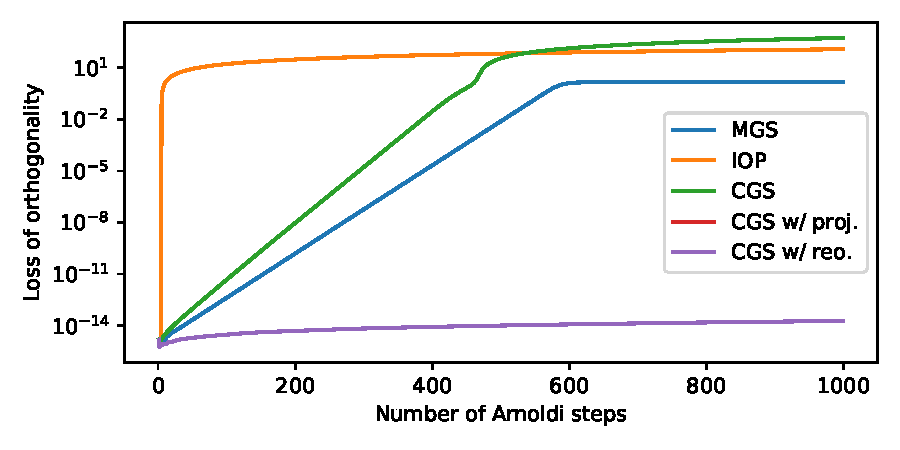
\includegraphics[width=\textwidth]{loss_of_orthogonality_grcar}
    \captionof{figure}{Loss of orthogonality $\norm{I_m - Q_m^T Q_m}_F$ of the Arnoldi basis vectors.}
\end{center}

For IOP, we choose to only orthogonalize against the two preceding vectors.
Thus, the runtime of IOP tells us how long the Lanczos algorithm would take if we used it on a similarly sized symmetric matrix.
However, for this matrix with this setting, IOP immediately loses orthogonality.
The Figure also shows that MGS is more stable than CGS, but the loss of orthogonality is only delayed by a few iterations.
However, reorthogonalization is very effective in maintaining the orthogonality of the basis vectors.
Noteably, it doesn't make a difference here whether we repeat CGS (\textsf{CGS w/ reo.}) or use the projection-based reorthogonalization of \verb|matfree| (\textsf{CGS w/ proj.}).

\begin{center}
    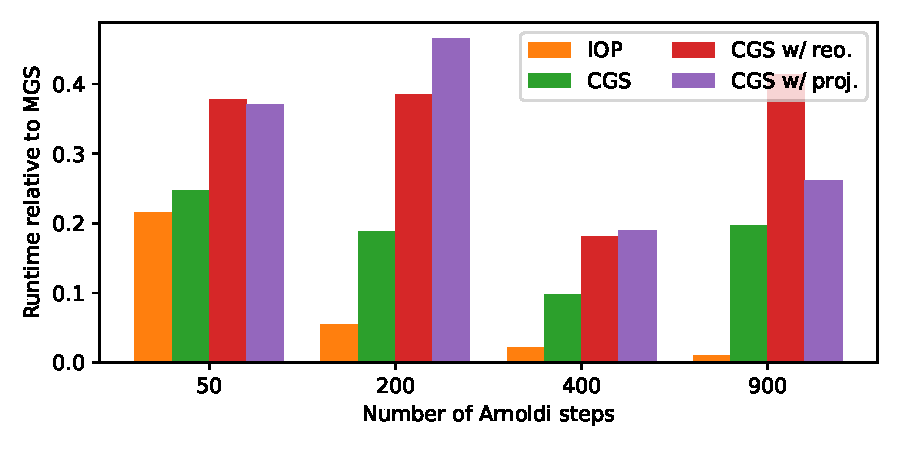
\includegraphics[width=\textwidth]{cpu_benchmark_grcar_rel}
    \captionof{figure}{Runtime generating $m$ Arnoldi vectors. Plotted is the time relative to what MGS takes.}
\end{center}

Next, we have a look at the runtime differences.
The Figure above plots the relative runtime of generating $m$ Arnoldi compared to using MGS.
The runtimes are chosen as the median of five tries.
Of course, a Numpy/ Scipy implementation will not have production level performance, but with the fast computational  BLAS kernels, it can point us towards the performance of the methods when hardware accelerators are available.
As we expect, MGS is consistently the slowest method.
Ignoring the inaccurate IOP, the fastest method is CGS but the really stable reorthogonalized versions are not much slower.
They both perform two additional matrix-vector products per iteration, so we would expect them to have very comparable runtimes.
Therefore, it is somewhat surprising that they differ this much at all.

As a last variation, we could try to see if one of these methods is more suitable for usage with a hardware accelerator.
For this, we use a free Google Colab notebook with a v4 TPU and reimplement the methods from above in JAX\@.
The JAX implementation is based on the code from \url{github.com/pnkraemer/matfree}.
Then we use the JAX JIT compiler to automatically take advantage of the TPU\@.
This is just a proof-of-concept and not meant to be truly representative of properly optimized performance, but we see the results in the table with minimal effort.
\begin{table}[ht]
\caption{Orthogonalization methods for $900$ Arnoldi vectors. Runtime is in seconds using TPU, loss of orthogonality is $\norm{I_m - Q_m^T Q_m}_F$, speedup is median $t_{\text{CPU}}/t_{\text{TPU}}$ of five runs.}
\begin{tabular}{lrrr}
    Variant & Runtime & Loss of orthogonality & Speedup\\\toprule
    MGS & 11.2 & 1.4 & 3.8\\
    CGS & 0.4 & 403.7 & 193\\
    CGS w/ proj. & 0.7 & $2\times10^{-14}$ & 94\\
\end{tabular}

\end{table}
Using the accelerator with activated double precision in JAX does not change the stability of the result, as expected.
However, we can mainly see that the reorthogonalization approach is much more able to take advantage of the TPU than the MGS approach.

\section{Further reading}
More thorough comparisons of orthogonalization procedures can be found in~\cite{tafollaLowsynchronizationArnoldiMethods2024, hernandezSLEPcTechnicalReport2007}.

\printbibliography


\end{document}